%\subsection{Jednowymiarowy torus}
%\label{alg:entorus_asynch_mesh}
%\begin{algorithm}[H]
%\SetKwInOut{Input}{Dane wejściowe}
%\SetKwInOut{Output}{Dane wyjściowe}
%\SetKwProg{ParFor}{parfor}{}{}
%\SetKwInOut{Help}{Dane pomocnicze}
%\Input{
%\begin{enumerate}
%\item podmacierze \(b=a\left((i-1)r+1\dots ir,1\dots n\right)\)
%\item \(r=\frac{n}{p}\)
%\item wektor \(x[1\dots n]\) umieszczone w procesorach \(P_i\) pracujących asynchronicznie, \(1\leq i  \leq p\) połączonych w pierścień
%\item zmienne lokalne w każdym procesorze \(P_i\) służace do przechowywania rozmiaru \(n\) oraz numeru procesora w postaci zmiennej \(i\)
%\end{enumerate}
%
%\Output{Iloczyn \(z=ax\) umieszczony w procesorze \(P_i\)}
%\Begin
%{
%\tcp*[f]{Oblczanie wektora \(y=bx\) przez procesory \(P_i, 1\leq i \leq p\)}\;
%
%\For{\(i=1 \quad \KwTo \quad n/p\)}
%{
%y[k]:=b[k,1]*x[1]\;
%\For{\(j:=1 \quad \KwTo \quad n\)}
%{
%y[k]:=y[k]+b[k,j]*x[j]\;
%}
%}
%\uIf{i:=1}{
%\(\mathtt{send}(y,prawy)\)\;
%}
%\Else{
%\(\mathtt{receive}(z[1..(i-1)r],lewy)\)\;
%\(z[1..ir]:=z[1..(i-1)]r\,||\,y\)\tcp*[f]{dopisanie wektora y}\;
%\(\mathtt{send}(z[1..ir],\,prawy)\)\;
%}
%\If{\(i=1\)}{
%\(\mathtt{receive}(z[1..n],\, lewy)\)\;
%\tcp*[f]{odebranie przez procesor \(P_1\) końcowego wyniku}\;
%}
%}
%}
%\caption{Algorytm mnożenia macierzy przez wektor w jednowymiarowym torusie}
%\end{algorithm}


% \subsection{Algorytm w dwuwymiarowym torusie}
% \begin{algorithm}[H]
% \SetKwFunction{Prawy}{prawy}
% \SetKwFunction{Dol}{dół}
% \SetKwInOut{Input}{Dane wejściowe}
% \SetKwInOut{Output}{Dane wyjściowe}
% \SetKwProg{ParFor}{parfor}{ do}{end}
% \SetKwInOut{Help}{Dane pomocnicze}
% %\begin{multicols*}{2}
% \Input{\begin{enumerate}
% \item macierze \(a\left[1..n,\,1..n\right]\) i \(b\left[1..n,\,1..n\right]\), których elementy \(a\left[i,\,j\right]\) umieszczone są w pamięciach lokalnych procesorów \(P_{i,j}\)
% \item zmienna lokalna w każdym procesorze służące do przechowyuwania rozmiaru \(n\)
% \item zmienne lokalne \(i\) oraz \(j\) przechowujące numer procesora
% \end{enumerate}
% }

% \Help{
% zmienna lokalna \(k\) w każdym procesorze \(P_{i,j}\)
% }
% \Output{
% \begin{enumerate}
% \item iloczyn macierzy \(c=ab\)
% \item elementy macierzy \(c[i,j]\) umieszczone w lokalnych zmiennych \(c\) procesorów \(P_{i,j}\)
% \end{enumerate}
% }
% %\end{multicols*}
% \Begin{
% \For{\(k:=2\) \To \(n\)}{
% \ParFor{\(P_{i,j},\, 1\leq i,\,j\leq n\) }{
% \If{\(k \leq i\) }{
% \(a\Longleftarrow\)\Prawy{\(a\)} \tcp*[r]{Przemieszczenie wierszy  \(a\)}
% \tcp*[r]{macierzy cyklicznie w lewo}
% }
% \If{\(k\leq j\)}{
% \(b\):=\Dol{\(b\)}\tcp*[f]{Przemieszczenie kolumn macierzy \(b\)}
% \tcp*[r]{cyklicznie w górę}
% }
% }
% }
% \tcp*[h]{Obliczanie iloczynu macierzy \(a\) i \(b\)}\;
% \For{\(k:=1\)\To \(n\)}{
% \ParFor{\(P_{i,j}, 1\leq i,\, j\leq n\)} {
% \uIf{\(k=1\)} {
% c:=a*b\;
% }
% \Else {
% a\(\Longleftarrow\)\Prawy{a}; b\(\Longleftarrow\)\Dol{b}; c:=c+a*b\;
% }
% }
% }
% }
% \end{algorithm}

% \subsection{Algorytm systoliczny w sieci dwuwymiarowej}

% Rysunek \ref{fig:systolic_mesh} przedstawia możliwy schemat obliczenia iloczynu \(AB = C\) w myśl paradygmatu systolicznego. Wiersze macierzy \(A\) są wprowadzane synchroniczne skośnie od lewej strony sieci; kolumny macierzy \(B\) są wprowadzane synchronicznie skośnie od góry sieci.\\
% Gdy procesor \(P_{i,j}\) odbierze dwie dane wejściowe \(A(i, l)\) i \(B(l,j)\), to przeprowadza operację \(C(i,j):=C(i,j+A(i,l)(B(l,j)\); po tym przesyła \(A(i,l)\) do swojego prawego sąsiada, a \(B(l,j)\) do sąsiada poniżej.

% Po \(O(n)\) krokach, każdy procesor \(P_{i,j}\) będzie miał szukaną wartość \(C(i,j)\).\\

% Algorytmy systoliczne pracują całkowicie synchronicznie; w każdej jednostce czasu, procesor otrzymuje dane od pewnego sąsiada, przeprowadza na nich lokalne obliczenia i następnie wysyła dane do któregoś swojego sąsiada.

% \begin{figure}[h]
% \centering
% 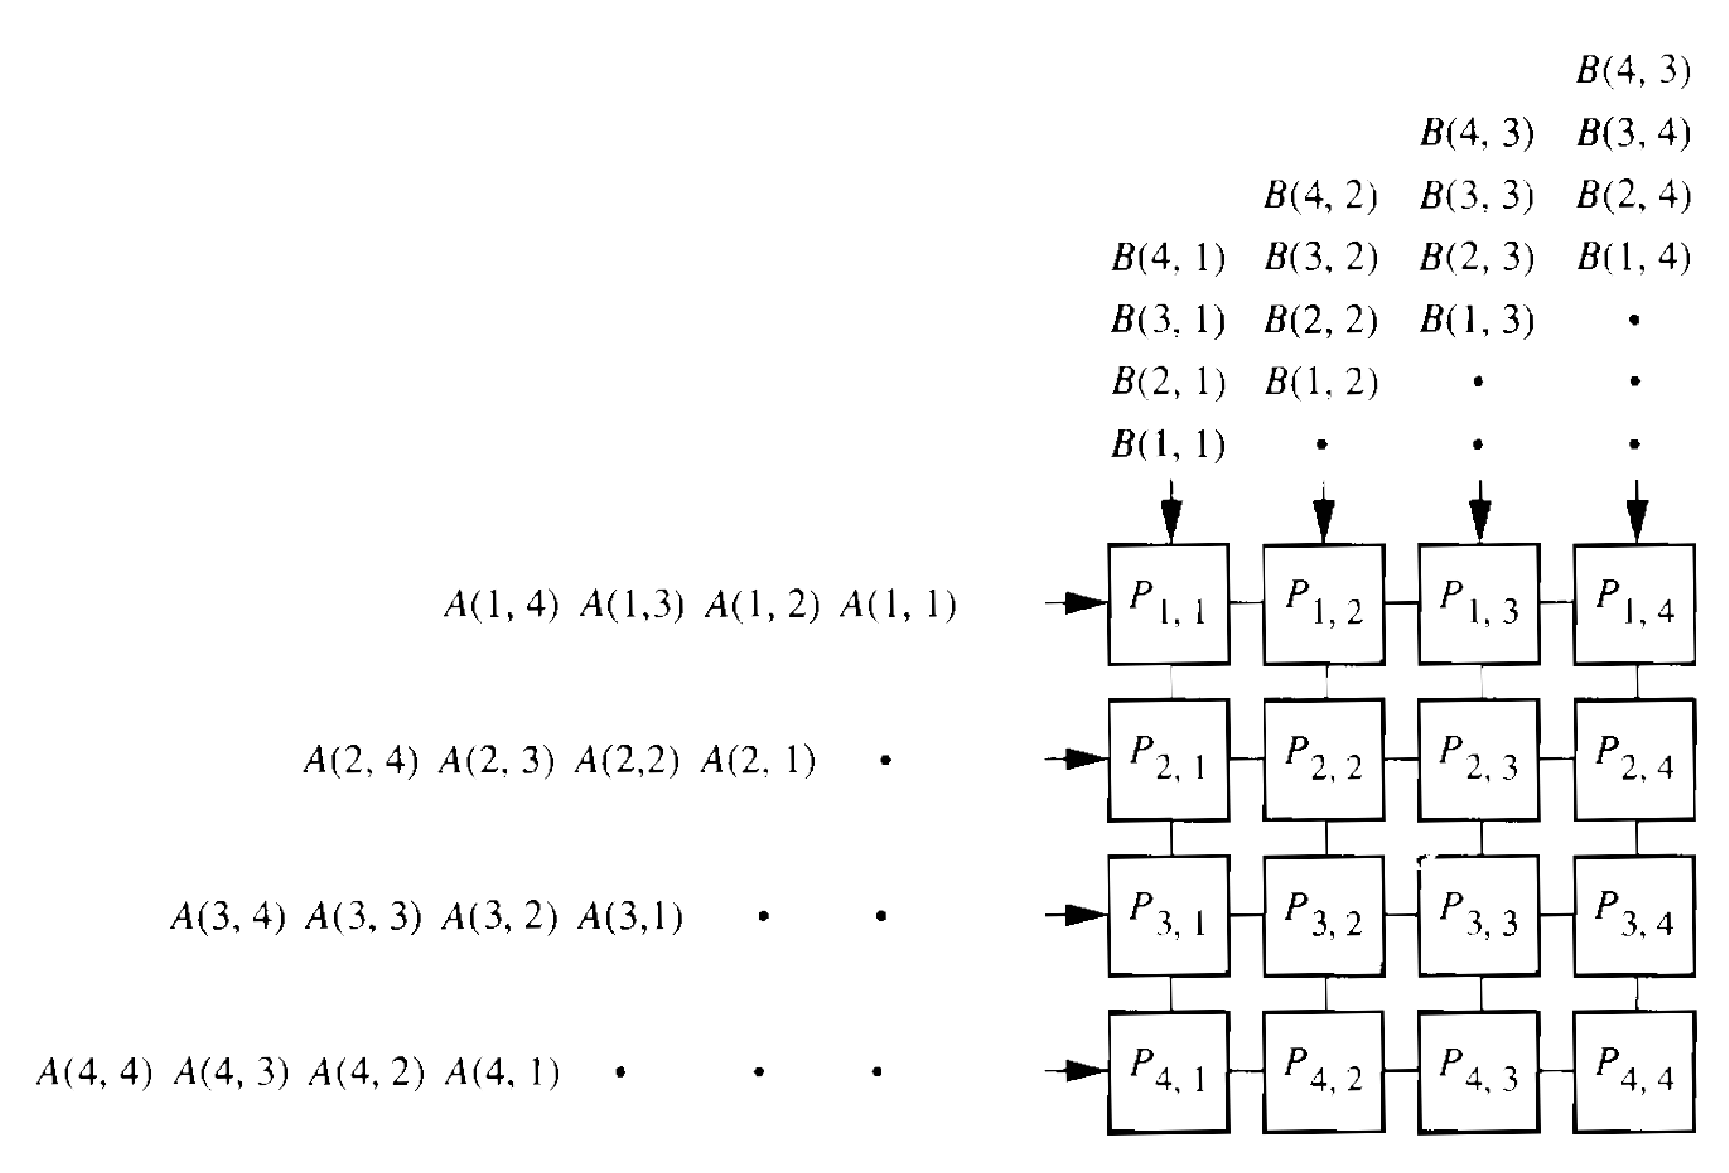
\includegraphics[width=30em]{images/systolic2.eps}
% \caption{Mnożenie macierzy w modelu sieciowym za pomocą algorytmu systolicznego. Wiersze macierzy \(\mathbf{A}\) są synchronicznie umieszczane w sieci od lewej strony, podczas, gdy równocześnie ,,od góry'' umieszczane są synchronicznie kolumny macierzy \(\mathbf{B}\). Gdy elementy \(A(i,l)\) i \(B(l,j)\) są dostępne na procesorze \(P_{i,j}\), wykonywane jest działanie \(C(i,j)=C(i,j)+A(i,l)B(l,j)\), \(A(i,l)\) zostaje wysłany do procesora \(P_{i,j+1}\) (o ile taki istnieje) oraz \(B(l,j)\) zostaje wysłany do procesora \(P_{i+1,j}\) (o ile taki istnieje).}
% \label{fig:systolic_mesh}
% \end{figure}

% \subsection{Algorytm w topologii hipersześcianu}
% \subsubsection{Rozgłaszanie ,,jednego do wszystkich'' w hipersześcianie}
% Rozważmy problem rozgłaszania elementu \(X\) przechowywanego w rejestrze \(D(0)\) procesora \(P_0\) do wszystkich procesorów \(P_i\) p-procesorowego hipersześcianu, gdzie \(p=2^d\).

% Algorytm polega na przechodzeniu z podkostek najniższego wymiaru, kolejno do najwyższego w \(d\) iteracjach. Pierwsza iteracja polega na wysłaniu kopii \(X\) przez procesor \(P_0\) do procesora \(P_1\). W drugiej iteracji procesor \(P_0\) i \(P_1\) wysyłają kopię \(X\) do \(P_2\) i \(P_3\) odpowiednio. Analogiczną operację przeprowadza się d-razy.


% % \begin{algorithm}\label{alg:broadcast_one_many}
% % \SetKwFunction{Prawy}{prawy}
% % \SetKwFunction{Dol}{dół}
% % \SetKwInOut{Input}{Dane wejściowe}
% % \SetKwInOut{Output}{Dane wyjściowe}
% % \SetKwProg{ParFor}{parfor}{ do}{end}
% % \SetKwInOut{Help}{Dane pomocnicze}
% % \Input{Procesor \(P_0\) z \(p=2^d\)-procesorowego synchronicznego hipersześcianu przechowuje element danych \(X\) w rejestrze \(D(0)\).}
% % \Output{\(X\) jest rogłaszany do wszystkich procesorów tak, że \(D(i)=X\), gdzie \(1\leq i \leq p-1\)}
% % \tcp*[l]{Algorytm dla procesora \(P_i\)}
% % \Begin{
% % \For{\(l=0\) \To \(d-1\)}{
% % \If{\(0\leq i \leq 2^l-1\)}{
% % Ustaw \(D(i^l):=D(i)\)\;
% % }
% % }
% % }
% % \caption{Algorytm rozgłaszania w sieci hipersześciennej}
% % \end{algorithm}


% Algorytm \ref{alg:broadcast_one_many} ma złożoność równoległą \(\mathcal{O}(\log{p})\)

% \subsubsection{Algorytm mnożenia}
% Rozważmy problem mnożenia macierzy \(AB = C\) w synchronicznym hipersześcianie z \(p=n^3\) procesorów, gdzie wszystkie macierze są wymiaru \(n\times n\).\\
% Niech \(n=2^q\) i stąd \(p=2^{3q}\). Przypiszmy procesorom indeksy \((l,i,j)\) takie, że \(P_{l,i,j}\) oznacza procesor \(P_r\), gdzie \(r=ln^{2}+in+j\). Innymi słowy, rozkładając indeks \(r\) binarnie otrzymuje, że \(q\) najbardziej znaczących bitów odpowiada indeksowi \(l\), następne \(q\) najbardziej znaczących bitów odpowiada indeksowi \(i\) i ostatecznie \(q\) najmniej znaczących bitow odpowiada wskaźnikowi \(j\). W szczególności, jeśli ustalimy dowolną parę wskaźników spośród \(l\), \(i\) oraz \(j\) oraz będziemy przechodzili z pozostałym wskaźnikiem po wszystkich jego możliwych wartościach, otrzymamy podkostkę wymiaru \(q\).\\

% Wejściowy ciąg \(A\) jest zapamiętany w podkostce wyznaczonej przez procesory \(P_{l,i,0}\), gdzie \(0\leq l, i \leq n-1\), tak, że \(A(i,l)\) jest zapamiętane w procesorze \(P_{l,i,0}\).\\
% Podobnie ciąg B jest zapamiętany w podkostce procesorów \(P_{l,0,j}\), gdzie procesor \(P_{l,0,j}\) zapamiętuje \(B(l,j)\).\\
% Celem jest obliczeniem \(C(i,j)=\sum_{l=0}^{n-1}A(i,l)B(l,j)\) dla \(0\leq i, j\leq n-1\). Algorytm składa się z trzech etapów:
% \begin{enumerate}
%  \item Dane wejściowe są rozdystrybuowane tak, że procesor \(P_{l,i,j}\) pamięta \(A(i,l)\) i \(B(l,j)\) dla \(0\leq l, i, j \leq n-1\).
%  \item Procesor \(P_{l,i,j}\) oblicza iloczyn \(C'(l,i,j)=A(i,l)B(l,j)\) dla wszystkich \(0\leq i, j, l \leq n-1\).
%  \item Dla wszystkich \(0\leq i, j \leq n-1\) procesorów \(P_{l,i,j}\), gdzie \(0\leq l\leq n-1\), obliczają sumę \(C(i,j)=\sum_{i=0}^{n-1} C'(l,i,j)\)
% \end{enumerate}

% Implementacja pierwszego etapu składa się z dwóch części. W pierwszej z nich \emph{rozgłaszamy}, dla każdego \(i, l, A(i,l)\), z procesora \(P_{i,l,0}\) do \(P_{l,i,})\) dla \(0\leq j \leq n-1\). Ponieważ zbiór procesorów \(\{P_{l,i,j}|0\leq j \leq n-1\}\) wyznacza q-wymiarową kostkę dla każdej z par \(i\) oraz \(l\), możemy użyć \textbf{algorytmu rozgłaszania}, żeby rozgłosić \(A(i,l)\) od procesora \(P_{l,i,0}\) do wszystkich procesorów \(P_{l,i,j}\).
% W drugiej części każdy element \(B(l,j)\) przechowywany w procesorze \(P_{l,0,j}\) jest rozgłaszany do procesorów \(P_{l,i,j}\) dla wszystkich \(0\leq i \leq n-1\). Pod koniec procesor \(P_{l,i,j}\) będzie przechowywał dwie wartości: \(A(i,l)\) i \(B(l,j)\). Używając algorytmu (tutaj referencja) etap pierwszy ma równoległą złożonośc czasową \(O(\log{n})\).

% Drugi etap polega na wykonywaniu pojedyńczych mnożeń na każdym z procesorów \(P_{l,i,j}\). Stąd etap na etap ten składa się tylko jeden równoległy krok obliczeniowy. Pod koniec procesor \(P_{l,i,j}\) przechowuje \(C'(l,i,j)\).

% Trzeci etap polega na obliczeniu \(n^2\) sum \(C(i,j)\). Wartości \(C'(l,i,j)\) każdej z sum znajudują się w q-wymiarowym hipersześcianie \(\{P_{l,i,j}\,|\,0\leq l\leq n-1\}\). Obliczanie takich sum ma równoległą złożoność czasową \(O(\log{n}\). Procesor \(P_{0,i,j}\) będzie przechowywał wartość \(C(i,j)\) iloczynu.

% Wobec powyższych iloczyn macierzy wymiaru \(n \times n\) w sieci hipersześciennej może być obliczony w czasie \(O(\log{n})\) dysponując \(n^3\) procesorami.
% \subsection{Algorytm Cannona w dwuwymiarowej sieci}
% \cite{communication_efficient}
% \subsection{Algorytm 2.5D}
% \cite{Solomonik:EECS-2011-72}
% \subsection{Algorytm 3D}
% \cite{communication_efficient}
% \subsection{Równoległy algorytm Strassena CAPS}
% \cite{DBLP:journals/corr/abs-1202-3173}

\subsection{Algorytm Cannona w dwuwymiarowym torusie}
Powiedzmy, że chcemy przeprowadzić obliczenie \(D = C + AB\) gdzie \(A, B, C\in\mathbb{R}^{n\times n}\) w dwuwymiarowym torusie o rozmiarach \(p_1 \times p_1\) oraz, że \(n=rp_1\). Macierze \(A=(A_{ij})\), \(B=(B_{ij})\), \(C=(C_{ij})\) możemy rozpatrywać jako macierze blokowe, gdzie \(A_{ij}\), \(B_{ij}\), \(C_{ij}\) są macierzami \(r\times r\). Przyjmijmy, że węzeł \(P_{ij}\) zawiera blok \(A_{ij}\), \(B_{ij}\) i \(C_{ij}\) oraz, że jego zadanie polega na nadpisywaniu macierzy \(C_{ij}\) poprzez
\begin{align*}
D_{ij}=C_{ij} + \sum_{k=1}^{p_1} A_{ik}B_{kj}.
\end{align*}

Zanim przejdziemy do przypadku ogólnego, pokażemy algorytm dla przypadku \(p_1 = 3\). Rozważmy sieć w topologii dwuwymiarowego torusa \(3\times 3\) (rys. \ref{fig:cannon_torus1}).

\begin{figure}[h]
\centering
\begin{tabular}{|C{1.5cm}|C{1.5cm}|C{1.5cm}|}
\hline
\(P_{11}\) & \(P_{12}\) & \(P_{13}\) \\
\hline
\(P_{21}\) & \(P_{22}\) & \(P_{23}\) \\
\hline
\(P_{31}\) & \(P_{32}\) & \(P_{33}\) \\
\hline
\end{tabular}
\caption{Węzły w dwuwymiarowym torusie \(3\times 3\)}
\label{fig:cannon_torus1}
\end{figure}

\noindent Weźmy pod uwagę wyłącznie aktywność na węźle \(P_{11}\). Wykonuje on obliczenie

\begin{align}\label{eq:cannon_torus1}
D_{11}=C_{11}+A_{11}B_{11} + A_{12}B_{21} + A_{13}B_{31}.
\end{align}

\noindent Załóżmy, że rozmieściliśmy sześć podmacierzy \(A\) i \(B\) tak jak na rysunku \ref{fig:cannon_torus2}.

\begin{figure}[h]
\centering
\begin{tabular}{|cc|cc|cc|}
\hline
\(A_{11}\) & \(B_{11}\) & \(A_{12}\) & \(-\) & \(A_{13}\) & \(-\) \\
\hline
\(-\) & \(B_{21}\) & \(-\) & \(-\) & \(-\) & \(-\) \\
\hline
\(-\) & \(B_{31}\) & \(-\) & \(-\) & \(-\) & \(-\) \\
\hline
\end{tabular}
\caption{Wstępne rozmieszczenie macierzy blokowych \(A_{ij}\) i \(B_{ij}\) koniecznych do wykonania algorytmu tylko na węźle \(P_{11}\). Miejsca oznaczone znakiem ,,\(-\)'' w ogólności są przeznaczone dla pozostałych danych. Rozmieszczenie danych w sieci odpowiada rysunkowi 
\ref{fig:cannon_torus1}}
\label{fig:cannon_torus2}
\end{figure}

\noindent Algorytm polega na przesuwaniu wierszy powstałych z bloków macierzy zapisanych w węzłach sieci. W każdym kroku na wybranym dla przykładu węźle \(P_{11}\) wykonujemy lokalne obliczenia prowadzące do otrzymania wartości wyrażenia \eqref{eq:cannon_torus1}. Kolejne kroki algorytmu przedstawione są na rysunku \ref{fig:cannon_torus3}.


\begin{figure}[h]
\centering
\begin{tabular}{lr}
\begin{tabular}{|cc|cc|cc|}
\hline
\(A_{12}\) & \(B_{21}\) & \(A_{13}\) & \(-\) & \(A_{11}\) & \(-\) \\
\hline
\(-\) & \(B_{31}\) & \(-\) & \(-\) & \(-\) & \(-\) \\
\hline
\(-\) & \(B_{11}\) & \(-\) & \(-\) & \(-\) & \(-\) \\
\hline
\end{tabular} &
\hspace{1cm}\(C_{loc}=C_{loc}+A_{12}B_{21}\)
\end{tabular}

\vspace{0.5cm}

\begin{tabular}{lr}
\begin{tabular}{|cc|cc|cc|}
\hline
\(A_{13}\) & \(B_{31}\) & \(A_{11}\) & \(-\) & \(A_{12}\) & \(-\) \\
\hline
\(-\) & \(B_{11}\) & \(-\) & \(-\) & \(-\) & \(-\) \\
\hline
\(-\) & \(B_{21}\) & \(-\) & \(-\) & \(-\) & \(-\) \\
\hline
\end{tabular} &
\hspace{1cm}\(C_{loc}=C_{loc}+A_{13}B_{31}\)
\end{tabular}

\vspace{0.5cm}

\begin{tabular}{lr}
\begin{tabular}{|cc|cc|cc|}
\hline
\(A_{11}\) & \(B_{11}\) & \(A_{12}\) & \(-\) & \(A_{13}\) & \(-\) \\
\hline
\(-\) & \(B_{21}\) & \(-\) & \(-\) & \(-\) & \(-\) \\
\hline
\(-\) & \(B_{31}\) & \(-\) & \(-\) & \(-\) & \(-\) \\
\hline
\end{tabular} &
\hspace{1cm}\(C_{loc}=C_{loc}+A_{11}B_{11}\)
\end{tabular}
\caption{Rozmieszczenie danych po wykonaniu trzech kroków metody Cannona z uwzględnienem danych koniecznych do obliczeń tylko na węźle \(P_{11}\)}
\label{fig:cannon_torus3}
\end{figure}

\noindent Po wykonaniu trzech kroków węzeł \(P_{11}\) ma w pamięci lokalnej macierz \(D_{11}\).

Przepływ danych został zorganizowany w taki sposób, że bloki \(A_{ij}\) przesuwanę są w siatce z prawej na lewą, zaś bloki \(B_{ij}\) --- z dołu na górę. Widać, że węzeł \(P_{11}\) musi wykonywać algorytm \ref{alg:cannon_1}.

\alglanguage{pseudocode}
\begin{algorithm}[H]
\centering
\begin{algorithmic}[1]
% \Input{macierze \(a[1\dots n, 1\dots n]\) i \(b[1\dots n, 1 \dots n]\) umieszczone w pamięci wspólnej modelu CREW PRAM o \(n^3\) procesorach; zmienne lokalne służące do przechowywania rozmiaru \(n\), gdzie (\(n=2^r\) dla pewnego \(0<r\in \mathbb{Z}\)); numer procesora w postaci zmiennych \(i\), \(j\) oraz \(k\)}
% \Tmp{macierz \(t[1\dots n, 1\dots, n, 1\dots, n]\) umieszczona w pamięci wspólnej; zmienna lokalna \(l\)}
% \Output{iloczyn macierzy \(c=ab\) w pamięci współdzielonej}
% \item[]
\For{\(i \gets 1, 3\)}
\Send{\(A_{loc}\), lewo}
\Send{\(B_{loc}\), góra}
\Recv{\(A_{loc}\), prawo}
\Recv{\(B_{loc}\), dół}
\State \(C_{loc} = C_{loc} + A_{loc}B_{loc}\)
\EndFor
\end{algorithmic}
\caption{Algorytm Cannona dla dwuwymiarowego torusa \(3\times 3\)}
\label{alg:cannon_1}
\end{algorithm}

\noindent W przyjętym modelu obliczeń zadziała również algorytm \ref{alg:cannon_2}:

\alglanguage{pseudocode}
\begin{algorithm}[H]
\centering
\begin{algorithmic}[1]
% \Input{macierze \(a[1\dots n, 1\dots n]\) i \(b[1\dots n, 1 \dots n]\) umieszczone w pamięci wspólnej modelu CREW PRAM o \(n^3\) procesorach; zmienne lokalne służące do przechowywania rozmiaru \(n\), gdzie (\(n=2^r\) dla pewnego \(0<r\in \mathbb{Z}\)); numer procesora w postaci zmiennych \(i\), \(j\) oraz \(k\)}
% \Tmp{macierz \(t[1\dots n, 1\dots, n, 1\dots, n]\) umieszczona w pamięci wspólnej; zmienna lokalna \(l\)}
% \Output{iloczyn macierzy \(c=ab\) w pamięci współdzielonej}
% \item[]
\For{\(i \gets 1, 3\)}
\Send{\(A_{loc}\), lewo}
\Recv{\(A_{loc}\), prawo}
\Send{\(B_{loc}\), góra}
\Recv{\(B_{loc}\), dół}
\State \(C_{loc} = C_{loc} + A_{loc}B_{loc}\)
\EndFor
\end{algorithmic}
\caption{Algorytm Cannona dla dwuwymiarowego torusa \(3\times 3\)}
\label{alg:cannon_2}
\end{algorithm}

Wykonanie algorytm \ref{alg:cannon_2} trwa nieco dłużej ze względu zatrzymanie wykonania programu dopóki macierz \(A_{loc}\) nie zostanie wysłana\footnote{W interfejsie MPI obydwa algorytmy traktowane literalnie wywołują zazębienie (ang. \emph{deadlock}) ze względu na blokującą funkcję MPI\_Send; istnieje szereg metod nieblokujących pozwalających na implementację obydwu algorytmów.}.

Rozważymy teraz aktywność węzłów \(P_{12}\), \(P_{13}\), \(P_{21}\), \(P_{31}\). W dotychczasowych roważaniach odpowiednio pomagały one jedynie w przesuwaniu bloków \(A_{11}\), \(A_{12}\), \(A_{13}\) oraz \(B_{11}\), \(B_{21}\) i \(A_{31}\). Gdyby \(B_{32}\), \(B_{12}\), \(B_{22}\) przechodziły przez węzeł \(P_{12}\) w trakcie wykonywania algorytmu, wówczas moglibyśmy na węźle \(P_{12}\) otrzymać wartość wyrażenia
\begin{align*}
D_{12} = C_{12} + A_{13}B_{32} + A_{11}B_{12} + A_{12}B_{22}.
\end{align*}

Rozumując podobnie, węzeł \(P_{13}\) mógłby obliczać wyrażenie
\begin{align*}
D_{13} = C_{13} + A_{11}B_{13} + A_{12}B_{23} + A_{13}B_{33}.
\end{align*}
\noindent o ile \(B_{13}\), \(B_{23}\) i \(B_{33}\) znajdowałyby się na węźle odpowiednio dla kroków \(t=1, 2, 3\).
\begin{figure}[h]
\centering
\begin{tabular}{lr}
\begin{tabular}{|cc|cc|cc|}
\hline
\(A_{12}\) & \(B_{21}\) & \(A_{13}\) & \(B_{32}\) & \(A_{11}\) & \(B_{13}\) \\
\hline
\(-\) & \(B_{31}\) & \(-\) & \(B_{12}\) & \(-\) & \(B_{23}\) \\
\hline
\(-\) & \(B_{11}\) & \(-\) & \(B_{22}\) & \(-\) & \(B_{33} \) \\
\hline
\end{tabular} &
\hspace{1cm}\(t=1\)
\end{tabular}

\vspace{0.5cm}

\begin{tabular}{lr}
\begin{tabular}{|cc|cc|cc|}
\hline
\(A_{13}\) & \(B_{31}\) & \(A_{11}\) & \(B_{12}\) & \(A_{12}\) & \(B_{23}\) \\
\hline
\(-\) & \(B_{11}\) & \(-\) & \(B_{22}\) & \(-\) & \(B_{33}\) \\
\hline
\(-\) & \(B_{21}\) & \(-\) & \(B_{32}\) & \(-\) & \(B_{13} \) \\
\hline
\end{tabular} &
\hspace{1cm}\(t=2\)
\end{tabular}

\vspace{0.5cm}

\begin{tabular}{lr}
\begin{tabular}{|cc|cc|cc|}
\hline
\(A_{11}\) & \(B_{11}\) & \(A_{12}\) & \(B_{22}\) & \(A_{13}\) & \(B_{33}\) \\
\hline
\(-\) & \(B_{21}\) & \(-\) & \(B_{32}\) & \(-\) & \(B_{13}\) \\
\hline
\(-\) & \(B_{31}\) & \(-\) & \(B_{12}\) & \(-\) & \(B_{23} \) \\
\hline
\end{tabular} &
\hspace{1cm}\(t=3\)
\end{tabular}
\caption{Cośtam}
\end{figure}





%syf syf syf

\begin{figure}[h]
\centering
\begin{tabular}{lr}
\begin{tabular}{|cc|cc|cc|}
\hline
\(A_{11}\) & \(B_{11}\) & \(A_{12}\) & \(B_{22}\) & \(A_{13}\) & \(B_{33}\) \\
\hline
\(A_{22}\) & \(B_{21}\) & \(A_{23}\) & \(B_{32}\) & \(A_{21}\) & \(B_{13}\) \\
\hline
\(A_{33}\) & \(B_{31}\) & \(A_{31}\) & \(B_{12}\) & \(A_{32}\) & \(B_{23} \) \\
\hline
\end{tabular} &
\hspace{1cm}
\end{tabular}
\caption{Cośtam}
\end{figure}

%syf 2

\begin{figure}[H]
\centering
\begin{tabular}{lr}
\begin{tabular}{|cc|cc|cc|}
\hline
\(A_{12}\) & \(B_{21}\) & \(A_{13}\) & \(B_{32}\) & \(A_{11}\) & \(B_{13}\) \\
\hline
\(A_{23}\) & \(B_{31}\) & \(A_{23}\) & \(B_{12}\) & \(A_{22}\) & \(B_{23}\) \\
\hline
\(A_{31}\) & \(B_{11}\) & \(A_{32}\) & \(B_{22}\) & \(A_{33}\) & \(B_{33} \) \\
\hline
\end{tabular} &
\hspace{1cm}\(t=1\)
\end{tabular}
\vspace{0.5cm}

\begin{tabular}{lr}
\begin{tabular}{|cc|cc|cc|}
\hline
\(A_{13}\) & \(B_{31}\) & \(A_{11}\) & \(B_{12}\) & \(A_{12}\) & \(B_{23}\) \\
\hline
\(A_{21}\) & \(B_{11}\) & \(A_{22}\) & \(B_{22}\) & \(A_{23}\) & \(B_{33}\) \\
\hline
\(A_{32}\) & \(B_{21}\) & \(A_{33}\) & \(B_{32}\) & \(A_{31}\) & \(B_{13} \) \\
\hline
\end{tabular} &
\hspace{1cm}\(t=2\)
\end{tabular}
\vspace{0.5cm}

\begin{tabular}{lr}
\begin{tabular}{|cc|cc|cc|}
\hline
\(A_{11}\) & \(B_{11}\) & \(A_{12}\) & \(B_{22}\) & \(A_{13}\) & \(B_{33}\) \\
\hline
\(A_{22}\) & \(B_{21}\) & \(A_{23}\) & \(B_{32}\) & \(A_{21}\) & \(B_{13}\) \\
\hline
\(A_{33}\) & \(B_{31}\) & \(A_{31}\) & \(B_{12}\) & \(A_{32}\) & \(B_{23} \) \\
\hline
\end{tabular} &
\hspace{1cm}\(t=3\)
\end{tabular}

\caption{Cośtam}
\end{figure}